\subsection{Vorbereitungsaufgabe}
\subsubsection{Rechteckspannung}
Die Rechteckspannung kann als
\begin{equation*}
  f(x)=
    \begin{cases}
      1,   \quad &0<x<\pi\\
      -1,  \quad &\pi<x<2\pi\\
      0,   \quad &x=n\pi, n \in \mathbb{Z}
    \end{cases}
\end{equation*}
\\geschrieben werden.
Für die Koeffizienten $a_{0}$ und $a_{n}$ gilt $a_{0}=a_{n}= \SI{0}{}$, da die Rechteckspannung ungerade ist und somit keine Cosinusanteile enthält.
\\Für $b_{n}$ ergibt sich
\begin{align*}
  b_{n}
  &=\frac{2}{2 \pi}  \int_{0}^{2 \pi} \! f(x) \sin{(nx)} dx
   =\frac{1}{\pi} \left( \int_{0}^{\pi} \! (+1) \sin{(nx)} dx + \int_{\pi}^{2\pi} \! (-1) \sin{(nx)} dx \right)\\
  &=\frac{1}{\pi} \left( \left[-\frac{1}{n} \cos{(nx)} \right]_{0}^{\pi} + \left[ \frac{1}{n} \cos{(nx)} \right]_{\pi}^{2\pi} \right)\\
  &=\frac{1}{ \pi n} \left( -\cos{(n\pi)} + \cos{(0)} + \cos{(n 2\pi)} - \cos{(n\pi)}\right)
   =\frac{1}{ \pi n} \left( 2-2\cos{(n\pi)} \right)\\
  &=\frac{2}{ \pi n} \left( 1-\cos{(n\pi)} \right)
  =\begin{cases}
    \frac{2}{ \pi n} \left( 1-1 \right)                 = 0,                \quad &\text{n  \quad gerade}\\
    \frac{2}{ \pi n} \left( 1- \left(-1 \right) \right) = \frac{4}{\pi n},  \quad &\text{n  \quad ungerade.}\\
  \end{cases}
\end{align*}
\\Damit fällt die Amplitude A der Peaks im Linienspektrum der Rechteckspannung mit
\begin{equation}
  A_{n} \propto \frac{A_{1}}{n}, \quad n=3, 5, 9, ...
\end{equation}
\\ab.

\subsubsection{Dreieckspannung}
Die Dreieckspannung wird durch
\begin{equation*}
  f(x)= |x|, \quad -\pi \le x \le \pi
\end{equation*}
\\beschrieben.
Die Koeffizienten $b_{n}$ sind immer 0, da die Funktion gerade ist.
\\Die Koeffizienten $a_{n}$ berechnen sich durch
\begin{align*}
  a_{n}
  &=\frac{2}{2\pi} \int_{-\pi}^{\pi} \! |x| \cos{(nx)} dx
   =\frac{2}{\pi} \int_{0}^{\pi} \! x \cos{(nx)} dx
   =\frac{2}{\pi} \left[ \frac{1}{n^2}(\cos{(nx)}+nx \sin{(nx)}) \right]_{0}^{\pi}\\
  &=\frac{2}{\pi n^2} \left( \cos{(n \pi )}+n \pi \sin{(n \pi)} -  \cos{(0)} - 0\right)
   =\frac{2}{\pi n^2} \left( \cos{(n \pi )}+n \pi \sin{(n \pi)} -  1 \right)\\
  &=\begin{cases}
    \frac{2}{\pi n^2} \left( 1+ 0 -  1 \right)  = 0,                   \quad &\text{n  \quad gerade}\\
    \frac{2}{\pi n^2} \left( -1 +0 -  1 \right) = -\frac{4}{\pi n^2},  \quad &\text{n  \quad ungerade.}\\
  \end{cases}
\end{align*}
\\Der Koeffizient $a_{0}$ berechnet sich durch
\begin{equation*}
  a_{0}= \frac{1}{\pi} \int_{-\pi}^{\pi} \! |x| dx = \frac{2}{\pi} \int_{0}^{\pi} \! x dx = \frac{2}{\pi} \left[ \frac{x^2}{2} \right]_{0}^{\pi} = \pi.
\end{equation*}
\\Die Amplitude der Dreieckspannung fällt also mit
\begin{equation}
  A_{n} \propto -\frac{A_{1}}{n^2}, \quad n=3, 5, 9, ...
\end{equation}
\\ab.

\subsubsection{Sägezahnspannung}
Eine Sägezahnspannung wird durch
\begin{equation*}
  f(x)=\begin{cases}
  x, \quad -\pi < x < \pi\\
  0, \quad x=\pm \pi
  \end{cases}
\end{equation*}
\\charakterisiert. Die Koeffizienten $a_{n}$ sind durch die Punktsymmetrie der Funktion immer gleich 0.
\\Die Koeffizienten $b_{n}$ berechnen sich durch
\begin{align*}
  b_{n}
  &=\frac{2}{2\pi} \int_{-\pi}^{\pi} \! x \sin{(nx)} dx
   =\frac{1}{\pi} \int_{0}^{\pi} \! x \sin{(nx)} dx
   =\frac{2}{\pi} \left[ \frac{1}{n^2}(\sin{(nx)}-nx \cos{(nx)}) \right]_{0}^{\pi}\\
  &=\frac{2}{\pi n^2} \left( \sin{(n \pi)} - n \pi \cos{(n \pi)} - 0 +0 \right)
   =\begin{cases}
    \frac{2}{\pi n^2} \left( 0 - \pi n - 0 +0 \right) = -\frac{1}{n},          \quad &\text{n  \quad gerade}\\
    \frac{2}{\pi n^2} \left( 0 - (-\pi n) - 0 +0 \right) = \frac{1}{n},       \quad &\text{n  \quad ungerade.}\\
  \end{cases}
\end{align*}
\\Die Amplituden der Sägezahnspannung fallen mit folgender Proportionalität ab:
\begin{equation}
  A_{n} \propto
    \begin{cases}
      -\frac{A_{1}}{n},   \quad &n= 2, 4, 6, 8, 10...\\
      \frac{A_{1}}{n},  \quad &n= 3, 5, 7, 9...
    \end{cases}
\end{equation}


\subsection{Fourieranalyse}
Für die Fourier-Analyse wird das Linienspektrum einer einfachen periodischen Schwingung gemessen.
Die Amplituden der Maxima sind in den Tabellen \ref{tab:rechteck}, \ref{tab:dreieck} und \ref{tab:sägezahn} aufgeführt.
Die drei Messungen für Rechteck-, Dreieck- und Sägezahnspannungen werden alle mit einer Freqenz von $f = \SI{100e3}{Hz}$ durchgeführt.


\begin{table}[h!]
  \centering
  \caption{Messdaten zur Zerlegung einer Rechteckspannung}
  \label{tab:rechteck}
  \begin{tabular}{c c c c c}
    \toprule
    n & $A_n$/V & $\frac{A_{n}}{A_{1}}$ & $\frac{A_1}{n}$ & Abweichung\\
    \midrule

    1  & 334 & 1,000         & 334,0  & 0,00\\
    3  & 110 & 0,329  & 111,3  & 1,21\\
    5  & 70  & 0,209  & 66,8   & 4,79\\
    7  & 46  & 0,138  & 47,7   & 3,73\\
    9  & 38  & 0,114  & 37,1   & 2,39\\
    11 & 26  & 0,078  & 30,4   & 16,78\\
    13 & 26  & 0,078  & 25,7   & 1,20\\
    15 & 20  & 0,060  & 22,3   & 11,33\\
    17 & 18  & 0,054  & 19,7   & 9,15\\






























    \bottomrule
  \end{tabular}
\end{table}


\begin{table}[h!]
  \centering
  \caption{Messdaten zur Zerlegung einer Dreieckspannung}
  \label{tab:dreieck}
  \begin{tabular}{c c c c c}
    \toprule
    n & $A_n$/V & $\frac{A_{n}}{A_{1}}$ & $\frac{A_1}{n}$ & Abweichung\\
    \midrule

    1 & 220,00  & 1,000         &  220,0	   &  0,00 \\
    2 & 23,60   & 0,117 &  24,4	 &  3,58 \\
    3 & 8,80    & 0,040         &  8,8	   &  0,00 \\
    4 & 4,00    & 0,018 &  4,5	   &  12,24 \\
    5 & 2,80    & 0,013 &  2,7	   &  3,09 \\
    6 & 1,52    & 0,007 &  1,8	   &  19,62 \\
    7 & 1,36    & 0,006 &  1,3	   &  4,47 \\
    8 & 0,80    & 0,004 &  0,98	 &  22,22 \\




    \bottomrule
  \end{tabular}
\end{table}

\input{tabSägezahn.tex}

\newpage
\subsection{Fouriersynthese}
Die theoretischen Amplituden sind zusammen mit den experimentellen Amplituden und mit der Normierung auf den Anfangswert in den Tabellen \ref{tab:recht}, \ref{tab:drei} und \ref{tab:säg} eingtragen.
Die synthetisierten Graphen sind außerdem in Abbildung \ref{fig:rechteck}, \ref{fig:dreieck} und \ref{fig:sägezahn} aufgeführt.


\begin{table}[h!]
  \centering
  \caption{Messdaten zur synthetisierten Rechteckspannung}
  \label{tab:recht}
  \begin{tabular}{c c c }
    \toprule
$n$  & $A_{n, theo}$ & $A_{n, exp}$ \\
      & V           & V             \\

    \midrule


    1	& 0,572 	&  0,572	\\
    3	& 0,1906	&  0,1907	\\
    5	& 0,1144	&  0,1144	\\
    7	& 0,0817	&  0,0817	\\
    9	& 0,0635	&  0,0635	\\



    \bottomrule
  \end{tabular}
\end{table}

\begin{figure}[h!]
  \centering
  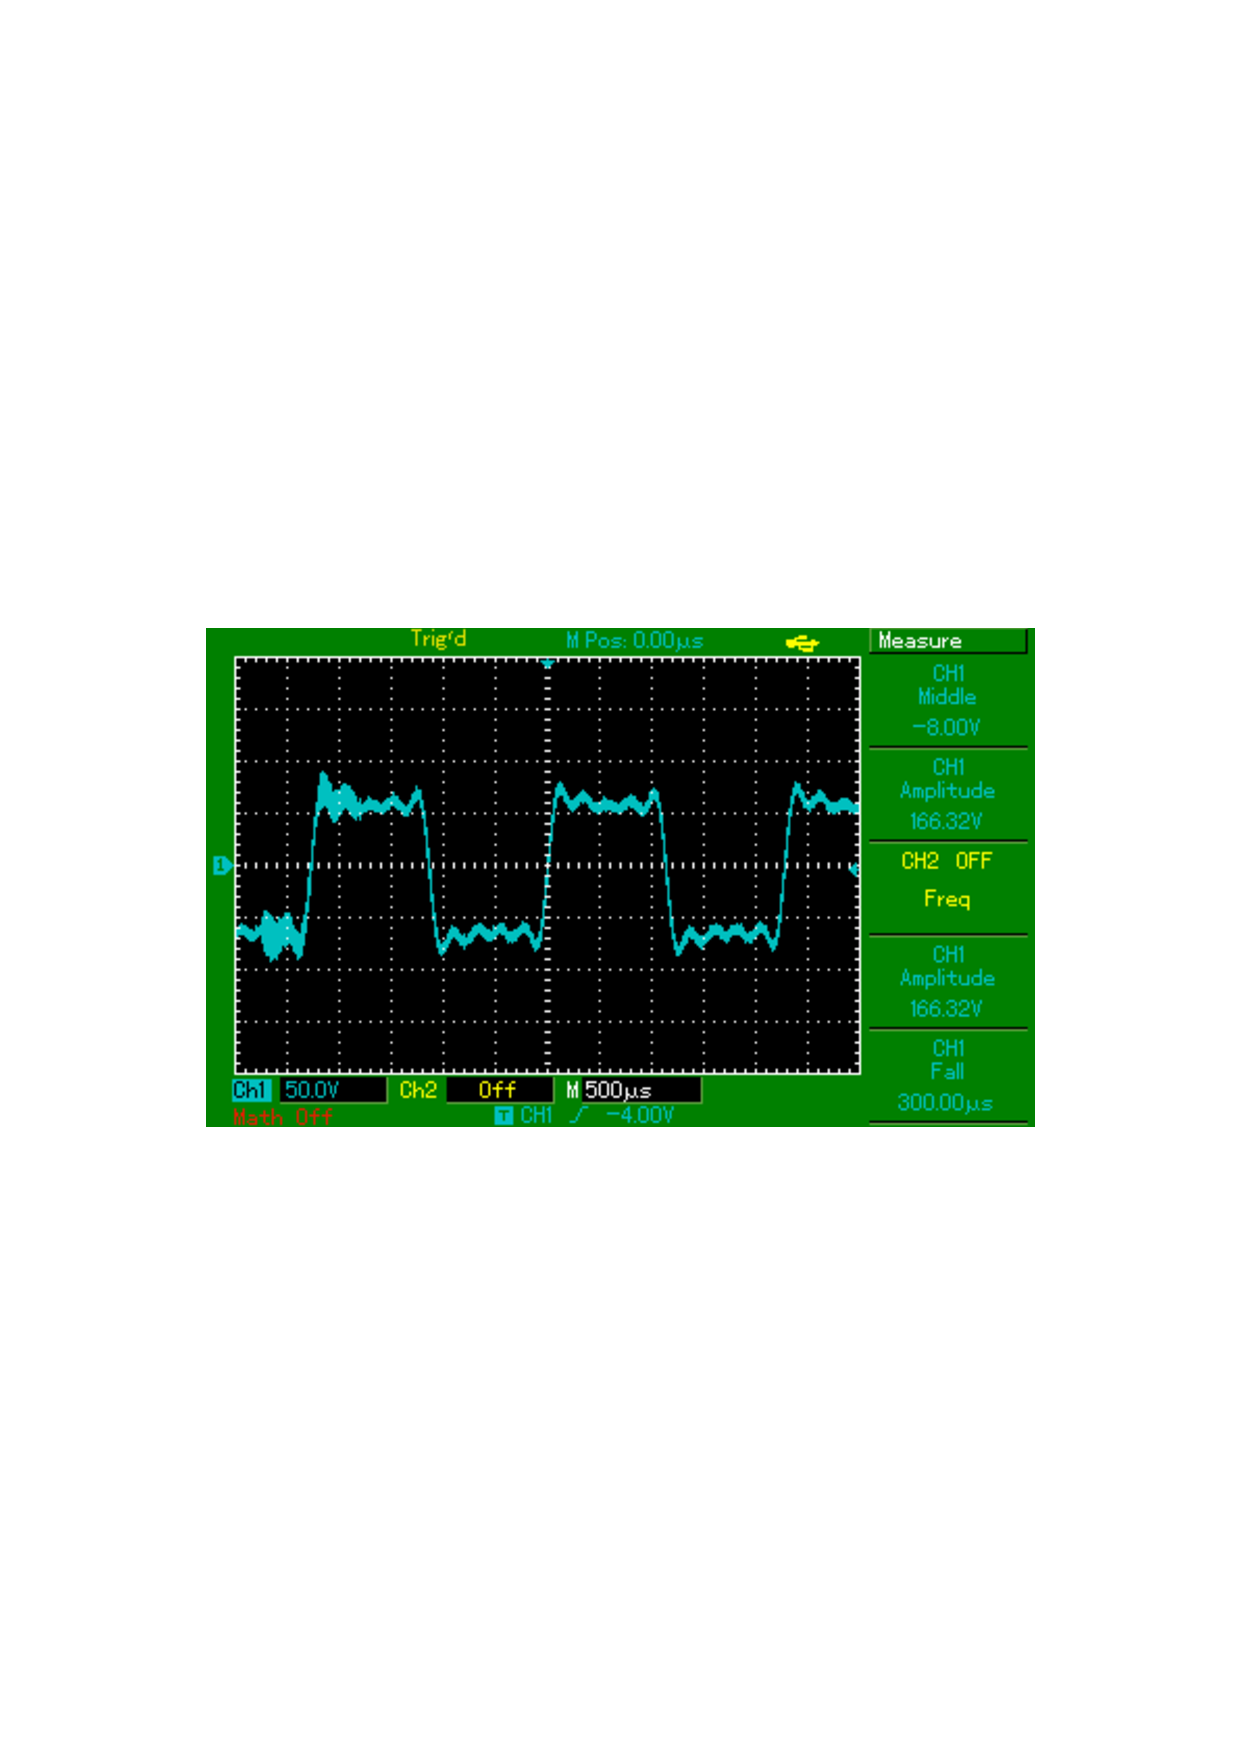
\includegraphics[width=\textwidth]{rechteck.pdf}
  \caption{Thermodruck der synthetisierten Rechteckspannung}
  \label{fig:rechteck}
\end{figure}


\begin{table}[h!]
  \centering
  \caption{Messdaten zur synthetisierten Dreieckspannung}
  \label{tab:drei}
  \begin{tabular}{c c c}
$n$  & $A_{n, theo}$ & $A_{n, exp}$ \\
      & V           & V               \\
    \midrule



    1	& 0,571	  & 0,571	 	\\
    3	& 0,0634	& 0,0634	\\
    5	& 0,0228	& 0,0229	\\
    7	& 0,0117	& 0,0118	\\
    9	& 0,0071	& 0,0072	\\




    \bottomrule
  \end{tabular}
\end{table}

\begin{figure}[h!]
  \centering
  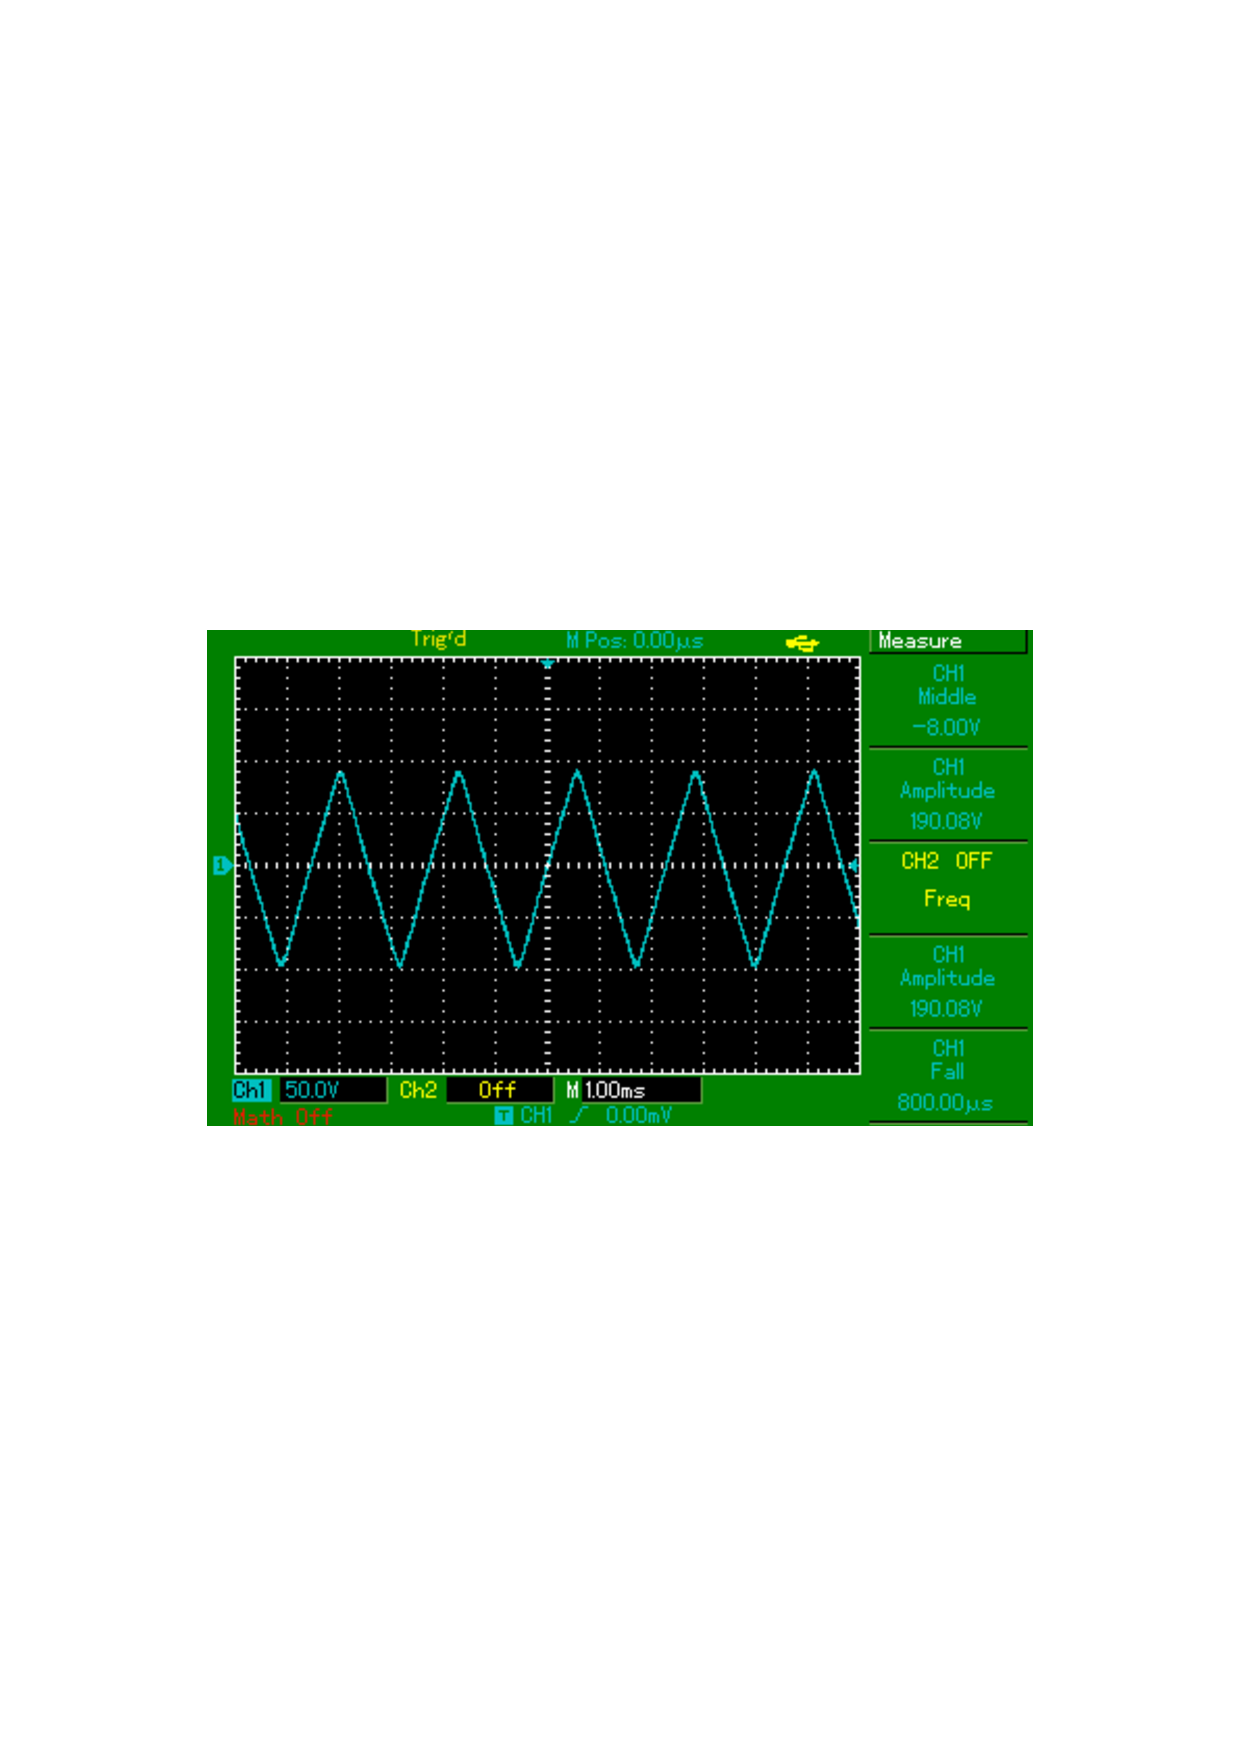
\includegraphics[width=\textwidth]{dreieck.pdf}
  \caption{Thermodruck der synthetisierten Dreieckspannung}
  \label{fig:dreieck}
\end{figure}


\begin{table}[h!]
  \centering
  \caption{Messdaten zur synthetisierten Rechteckspannung}
  \label{tab:säg}
  \begin{tabular}{c c c }
    \toprule
$n$  & $A_{n, theo}$ & $A_{n, exp}$ \\
      & V           & V               \\
    \midrule


    1	& 0,571 	&0,571	\\
    2	& 0,2855	&0,2855	\\
    3	& 0,1903	&0,1902	\\
    4	& 0,1426	&0,1456	\\
    5	& 0,1142	&0,1143	\\
    6	& 0,0952	&0,0952	\\
    7	& 0,0816	&0,0816	\\
    8	& 0,0714	&0,0714	\\
    9	& 0,0634	&0,0634	\\
    10&	0,0571	&0,0571	\\



    \bottomrule
  \end{tabular}
\end{table}

\begin{figure}[h!]
  \centering
  \includegraphics[width=\textwidth]{sägezahn.pdf}
  \caption{Thermodruck der synthetisierten Sägezahnspannung}
  \label{fig:sägezahn}
\end{figure}
\newpage
